\chapter{Проектирование системы дистрибуции программных модулей}
\label{cha:design}

Проектирование системы дистрибуции программных модулей - это сложная задача, ставка при которой делается не только на функциональность, но и на безопасность. 

\section{Анализ архитектуры современных систем}

Современная разработка ПО основывается на двух основных типах архитектуры: монолитной и микросервисной. Давайте кратко рассмотрим каждый из этих типов. 

Монолитная архитектура представляет собой классическую модель подхода к программному обеспечению, где используется один самостоятельный модуль, функционирующий отдельно от других приложений. Именно поэтому ее и называют "монолитной". Все фрагменты кода и бизнес-функции в такой архитектуре объединены в одной области.

\begin{figure}
  \centering
  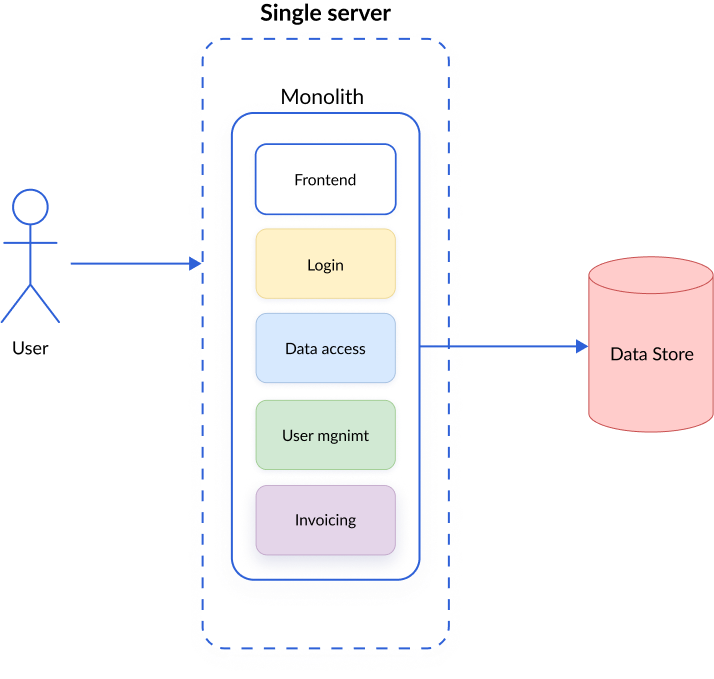
\includegraphics[width=.7\textwidth]{graphics/img/mono.png}
  \caption{Пример монолитной архитектуры}
  \label{fig:mono}
\end{figure}


Микросервисная архитектура - это разделение архитектуры на множество независимо функционирующих служб. Каждая из этих служб имеет свою бизнес-логику и систему управления базами данных (СУБД), служащую определенной цели. Оба эти типа архитектур стоит рассмотреть в контексте сравнения.

\begin{figure}
  \centering
  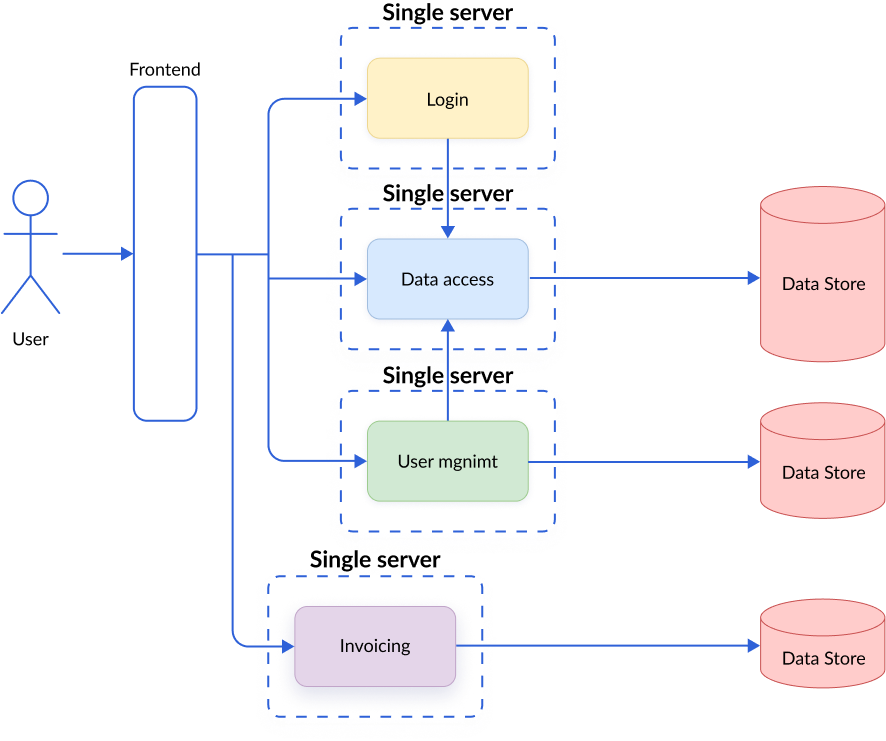
\includegraphics[width=.9\textwidth]{graphics/img/micro.png}
  \caption{Пример микросервисной архитектуры}
  \label{fig:micro}
\end{figure}

Среди недостатков монолитной архитектуры можно выделить плохую масштабируемость, трудность внедрения новых модулей и проблемы при обновлении технологий, так как это может затронуть весь проект, к тому же есть и проблемы с отказоустойчивостью и трудностью в горизонтальной масштабируемости. Однако она проще в развертывании, разработке, тестировании и отладке, чем микросервисная.

Микросервисная архитектура обладает гибкостью: каждая команда может разрабатывать и разворачивать свой сервис независимо, что ускоряет сроки реализации проектов и позволяет выбирать технологии согласно предпочтениям команды. Отказоустойчивость в данном случае - тоже немаловажный плюс, поскольку при сбое одного микросервиса функциональность приложения страдает лишь частично. Недостатками же можно считать большие затраты при разрастании приложения и сложность отладки и координации между разными командами.

Текущий проект работы подразумевает под собой максимальную нагрузку, портируемость и отказоустойчивость. С учетом этого, было решено использовать микросервисную архитектуру, да и существующие системы неспроста являются микросервисными, так как высокие требования делают зависимость от более гибкой системы.

\section{Функциональные возможности системы}

Выробатанными требованиями мы приходим к функциональным возможностям проектируемой системы:

\subsection{Серверная часть системы}

\begin{enumerate}
    \item Загрузка на сервер, отправка пакета (модуля) с сервера.
    \item Управление зависимостями модулей.
    \item Система версий модулей.
    \item Информирование о модулях и их безопасности.
    \item Аутефикация и авторизация на основе JWT.
    \item Реализация открытого API.
    \item Система блокировки и защиты особо критических модулей.
\end{enumerate}

\Abbrev{API}{Application Programming Interface}

\Define{API}{Application Programming Interface ""--- представляет собой набор правил и инструкций, согласно которым различные программы и сервисы могут общаться между собой. Эти правила определяют, как данные и функциональность могут быть переданы от одной программы к другой, как они могут взаимодействовать и обмениваться информацией}

\subsection{Клиентская часть системы}

\begin{enumerate}
    \item Простой и понятный интерфейс через CLI.
    \item Конфигурирование клиентской части.
    \item Управление установленными модулями, включая загрузку, обновление и удаление.
    \item Информирование о модулях и их безопасности.
\end{enumerate}

\section{Микросервис авторизации}

В предложенной работе необходимо разработать микросервис авторизации для системы. Он будет отвечать за следующие функции: 
- регистрацию пользователя; 
- аутентификацию и авторизацию пользователя с выдачей двух JWT (refresh, access); 
- обновление access JWT с помощью refresh JWT; 
- завершение сессии пользователя путем аннулирования двух JWT (refresh, access); 
- предоставление персональной информации пользователя после прохождения этапа авторизации;
- удаление пользователем своего личного аккаунта после прохождения этапа авторизации.

\Define{JWT}{JSON Web Token ""--- руководствующийся открытым стандартом (RFC 7519), представляет собой универсальное средство формирования токенов доступа, рснованный на надежном и широкораспространенном формате JSON, он стал одним из наиболее эффективных и безопасных способов обеспечения эффективной передачи информации между устройствами и серверами в кодированном виде}

%%% Local Variables:
%%% mode: latex
%%% TeX-master: "rpz"
%%% End:
